\documentclass[border=5pt]{standalone}
\usepackage{tikz}
\usetikzlibrary{positioning, calc, decorations.pathreplacing}
\usepackage{booktabs}
\usepackage{array}
\usepackage{amsmath,amssymb}

% Colors
\definecolor{cGreen}{HTML}{2E7D32}
\definecolor{cRed}{HTML}{C62828}
\definecolor{cGray}{HTML}{9E9E9E}
\definecolor{cBlue}{HTML}{1565C0}
\definecolor{cBg}{HTML}{F5F5F5}
\definecolor{cHighlight}{HTML}{E3F2FD}

% Symbols
\newcommand{\cmark}{\textcolor{cGreen}{$\checkmark$}}
\newcommand{\dash}{\textcolor{cGray}{\textendash}}
\newcommand{\best}[1]{\textbf{#1}}
\newcommand{\degr}[1]{\textcolor{cRed}{\footnotesize #1}}

\begin{document}
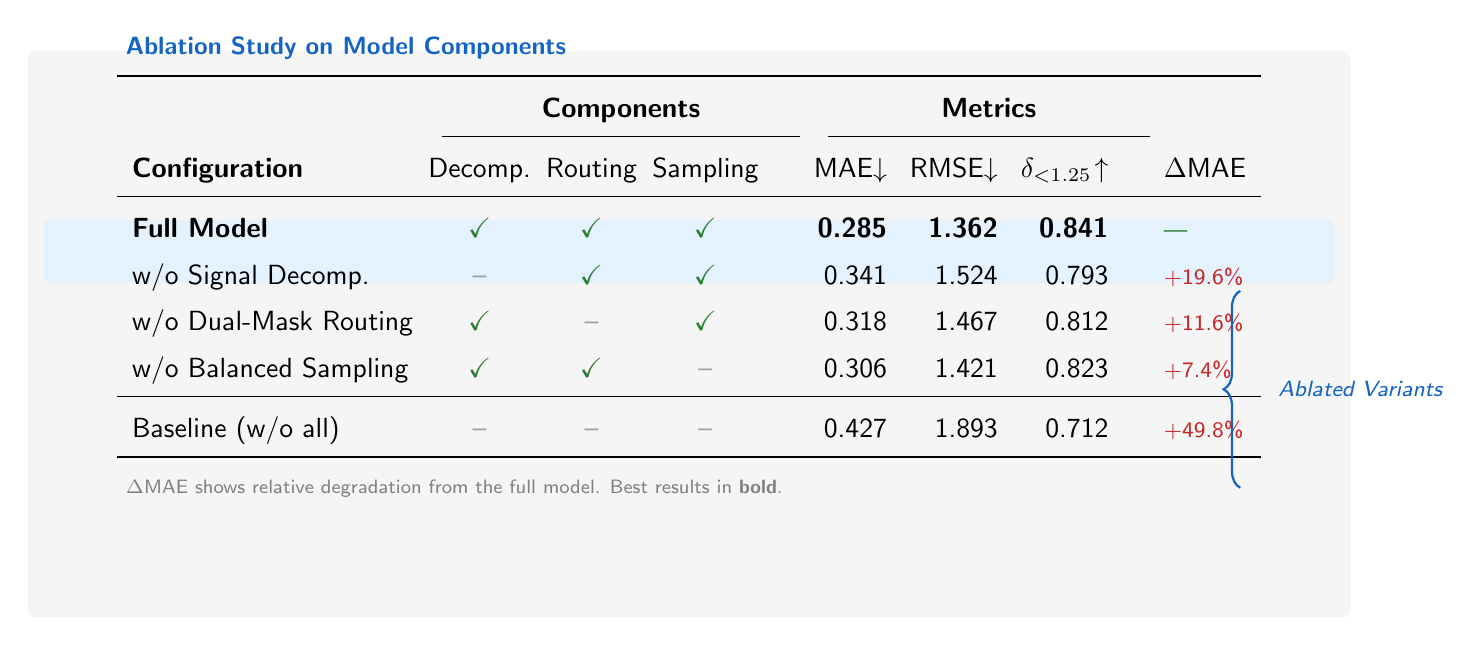
\begin{tikzpicture}[
  every node/.style={font=\sffamily},
  title/.style={font=\sffamily\small\bfseries, text=cBlue},
  note/.style={font=\sffamily\scriptsize, text=black!50},
]

% Background panel
\fill[cBg, rounded corners=3pt] (-0.4, -6.2) rectangle (16.4, 1.0);

% Highlight behind full model row
\fill[cHighlight, rounded corners=2pt] (-0.2, -1.15) rectangle (16.2, -1.95);

% Table as a node
\node[inner sep=0pt, anchor=north] (table) at (8, 0.7) {%
  \renewcommand{\arraystretch}{1.4}%
  \setlength{\tabcolsep}{4.5pt}%
  \begin{tabular}{@{\;\;}l @{\;\;} c @{\;\;} c @{\;\;} c @{\qquad} r @{\;\;\;} r @{\;\;\;} r @{\qquad} l@{\;\;}}
    \toprule
    & \multicolumn{3}{c}{\textbf{Components}} & \multicolumn{3}{c}{\textbf{Metrics}} & \\
    \cmidrule(lr){2-4} \cmidrule(lr){5-7}
    \textbf{Configuration} & Decomp. & Routing & Sampling
      & MAE$\downarrow$ & RMSE$\downarrow$ & $\delta_{<1.25}\!\uparrow$ & $\Delta$MAE \\
    \midrule
    \textbf{Full Model} & \cmark & \cmark & \cmark
      & \best{0.285} & \best{1.362} & \best{0.841} & \textcolor{cGreen}{\footnotesize ---} \\
    w/o Signal Decomp. & \dash & \cmark & \cmark
      & 0.341 & 1.524 & 0.793 & \degr{+19.6\%} \\
    w/o Dual-Mask Routing & \cmark & \dash & \cmark
      & 0.318 & 1.467 & 0.812 & \degr{+11.6\%} \\
    w/o Balanced Sampling & \cmark & \cmark & \dash
      & 0.306 & 1.421 & 0.823 & \degr{+7.4\%} \\
    \midrule
    Baseline (w/o all) & \dash & \dash & \dash
      & 0.427 & 1.893 & 0.712 & \degr{+49.8\%} \\
    \bottomrule
  \end{tabular}%
};

% Right-side brace for ablated variants
\draw[decorate, decoration={brace, amplitude=6pt, mirror}, thick, cBlue]
  (15.0, -2.05) -- (15.0, -4.55)
  node[midway, right=10pt, font=\sffamily\footnotesize\itshape, text=cBlue]
  {Ablated Variants};

% Title
\node[title, above=2pt of table.north west, anchor=south west]
  {Ablation Study on Model Components};

% Bottom note
\node[note, below=4pt of table.south west, anchor=north west]
  {$\Delta$MAE shows relative degradation from the full model. Best results in \textbf{bold}.};

\end{tikzpicture}
\end{document}